% A USV surveying the shipwreck model (spike/shipwreck, modeled on the Monohansett) with a downward profiling sonar
% and a sidescan on each side. Line art in the style of the sonar types figure (sonar_types.tex).
% Units are meters in the shipwreck model frame: +X toward the bow, +Y to port, z = 0 the seabed; water depth 8 m
% (shipwreck.md, decision 5). The vertical scale is exaggerated 2x.
% The USV is partway along a survey line at y = +7 (to port of the wreck), heading +X. Behind it: the sidescan swaths (shaded), the profiler
% soundings (dots, at the wreck's height) and the acoustic shadow the wreck casts away from the track.
% Build: pdflatex shipwreck_survey.tex, then pdftocairo to ../images/shipwreck_survey.{png,svg}
\documentclass[tikz,border=6pt]{standalone}
\usetikzlibrary{arrows.meta,calc}
\renewcommand{\familydefault}{\sfdefault}

\tikzset{
  lbl/.style={font=\sffamily\small},
  obl/.style={x={(0.2cm,0cm)},y={(0.09cm,0.1cm)},z={(0cm,0.4cm)}},
  edge/.style={thin},
  move/.style={thick,-{Latex[length=2.4mm]}},
  lead/.style={thin,black!70},
  declare function={
    % wreck height above the seabed, a coarse stand-in for the meshes, used for the soundings
    boil(\x,\y)=((\x>-4)&&(\x<0)&&(abs(\y)<1.5))*(1.8+sqrt(max(2.25-\y*\y,0)));
    eng(\x,\y)=((\x>-6.5)&&(\x<-4.5)&&(abs(\y)<1))*3.0;
    aft(\x,\y)=((\x>-16)&&(\x<1.5)&&(abs(\y)<4.5))*(1.0+(abs(\y)>3.5));
    mid(\x,\y)=((\x>2.5)&&(\x<19)&&(abs(\y)<4.8))*(0.4+((abs(\x-10)<4)&&(abs(\y)<3))*0.45);
    bow(\x,\y)=((\x>20)&&(\x<32.5)&&(abs(\y)<4.5*(32.5-\x)/12.5))*0.8;
    wh(\x,\y)=max(boil(\x,\y),eng(\x,\y),aft(\x,\y),mid(\x,\y),bow(\x,\y));
  },
}

% box with its visible faces filled: x0 x1 y0 y1 z0 z1 (y0 is the near side)
\newcommand{\cuboid}[6]{
  \draw[fill=black!15] (#1,#3,#6) -- (#2,#3,#6) -- (#2,#4,#6) -- (#1,#4,#6) -- cycle;
  \draw[fill=white] (#1,#3,#5) -- (#2,#3,#5) -- (#2,#3,#6) -- (#1,#3,#6) -- cycle;
  \draw[fill=white] (#2,#3,#5) -- (#2,#4,#5) -- (#2,#4,#6) -- (#2,#3,#6) -- cycle;
}

\begin{document}
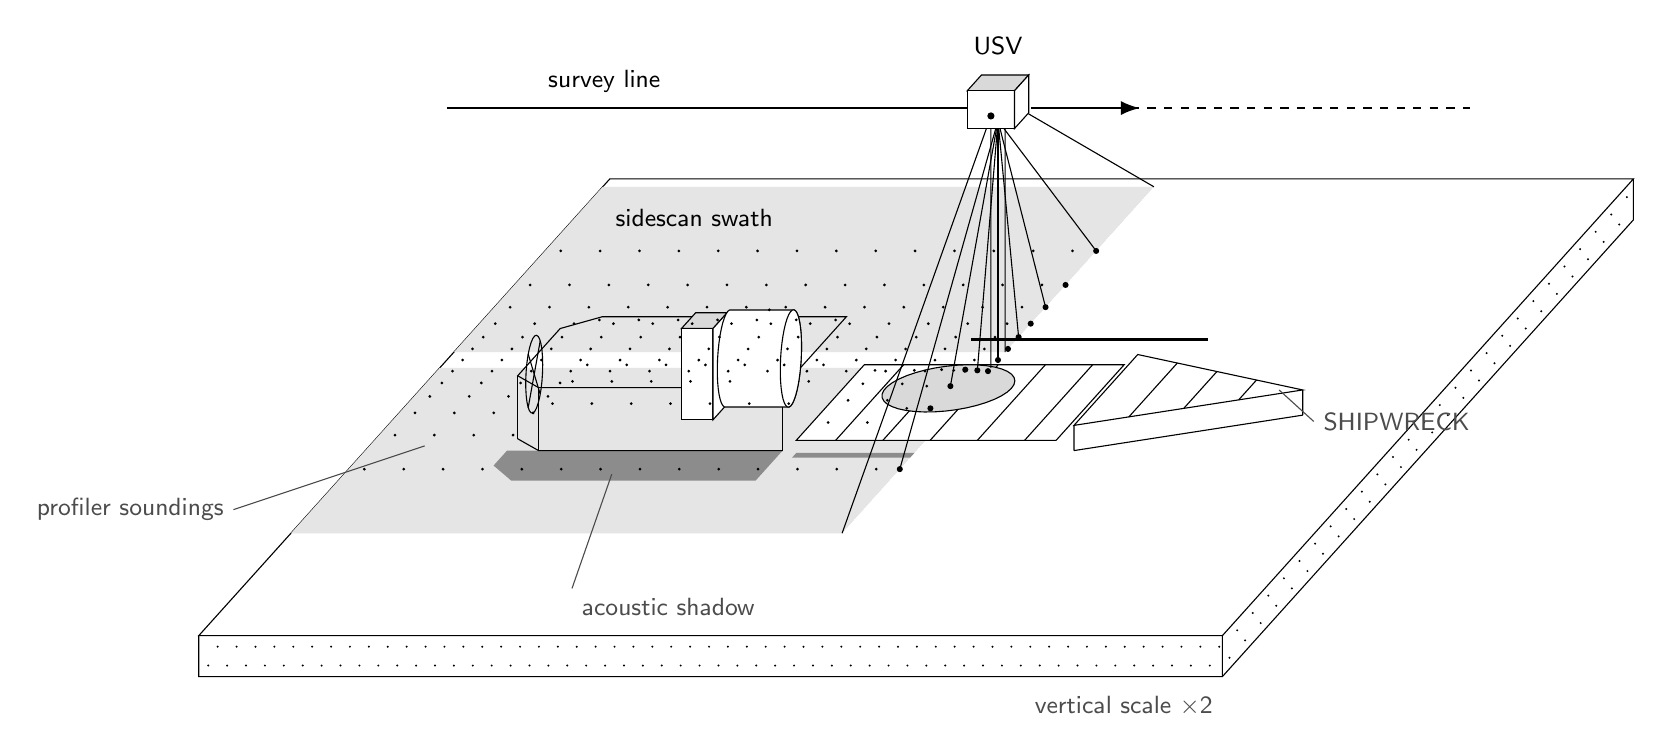
\begin{tikzpicture}[obl]
  \def\H{8}\def\yt{7}\def\xu{10}   % water depth, survey line (port of the wreck), USV position along it

  % ------------------------------------------------ seabed
  \draw[fill=white] (-25,-28,0) -- (40,-28,0) -- (40,30,0) -- (-25,30,0) -- cycle;
  \foreach \z [count=\i] in {-0.35,-0.95} {
    \pgfmathsetmacro{\o}{mod(\i,2)*0.6}
    \foreach \x in {-24.4,-23.2,...,39.5} \fill ({\x+\o},-28,\z) circle (0.4pt);
    \foreach \y in {-27,-24.8,...,29.5} \fill (40,{\y+\o*1.8},\z) circle (0.4pt);
  }
  \draw (-25,-28,0) -- (-25,-28,-1.3) -- (40,-28,-1.3) -- (40,30,-1.3) -- (40,30,0) (40,-28,0) -- (40,-28,-1.3);

  % ------------------------------------------------ what has been surveyed: swaths and shadow, up to the USV
  \begin{scope}
    \clip (-25,-28,0) -- (\xu,-28,0) -- (\xu,30,0) -- (-25,30,0) -- cycle;
    \fill[black!10] (-25,-15,0) -- (\xu,-15,0) -- (\xu,6,0) -- (-25,6,0) -- cycle;    % starboard sidescan swath
    \fill[black!10] (-25,8,0) -- (\xu,8,0) -- (\xu,29,0) -- (-25,29,0) -- cycle;      % port sidescan swath
    % acoustic shadow on the far side of the wreck from the track: y_end = yt - (yt - y_edge) * H / (H - height)
    \fill[black!45] (-16,-4.5,0) -- (1.5,-4.5,0) -- (1.5,-8.33,0) -- (-14,-8.33,0) -- (-16,-6.4,0) -- cycle;   % aft section, 2 m
    \fill[black!45] (2.5,-4.8,0) -- (19,-4.8,0) -- (19,-5.4,0) -- (2.5,-5.4,0) -- cycle;    % midships, 0.4 m
  \end{scope}

  % ------------------------------------------------ the wreck
  % fallen mast off the port side
  \draw[line width=1.2pt] (7.5,8.8,0.2) -- (22.5,8.8,0.2);
  % bow section, collapsed, 0.8 m
  \draw[fill=white] (20,-4.5,0.8) -- (32.5,0,0.8) -- (20,4.5,0.8) -- cycle;
  \draw (20,-4.5,0) -- (32.5,0,0) (20,-4.5,0) -- (20,-4.5,0.8) (32.5,0,0) -- (32.5,0,0.8);
  \foreach \x in {23,26,29} \draw[edge] (\x,{-4.5*(32.5-\x)/12.5},0.8) -- (\x,{4.5*(32.5-\x)/12.5},0.8);
  % midships, sides splayed flat, frames, coal mound
  \draw[fill=white] (2.5,-4.8,0.4) -- (19,-4.8,0.4) -- (19,4.8,0.4) -- (2.5,4.8,0.4) -- cycle;
  \foreach \x in {5,8,...,17} \draw[edge] (\x,-4.8,0.4) -- (\x,4.8,0.4);
  \draw[fill=black!15] plot[domain=0:360,samples=40] ({10+4*cos(\x)},{3*sin(\x)},0.85) -- cycle;
  % aft section: open hull 2 m proud, stern tapered
  \draw (-16,3,2) -- (-14,4.5,2) -- (1.5,4.5,2) -- (1.5,-4.5,2) -- (-14,-4.5,2) -- (-16,-3,2) -- cycle;
  \draw (-16,-3,0) -- (-14,-4.5,0) -- (1.5,-4.5,0);
  \draw (-16,-3,0) -- (-16,-3,2) (-14,-4.5,0) -- (-14,-4.5,2) (1.5,-4.5,0) -- (1.5,-4.5,2);
  % engine and boiler, the highest parts
  \cuboid{-6.5}{-4.5}{-1}{1}{0.1}{3.0}
  \draw[fill=white] plot[domain=81:261,samples=20] (-4,{1.5*cos(\x)},{1.8+1.5*sin(\x)})
        -- plot[domain=261:441,samples=20] (0,{1.5*cos(\x)},{1.8+1.5*sin(\x)}) -- cycle;
  \draw[fill=white] plot[domain=0:360,samples=40] (0,{1.5*cos(\x)},{1.8+1.5*sin(\x)}) -- cycle;
  % propeller at the stern
  \draw plot[domain=0:360,samples=30] (-16.3,{1.2*cos(\x)},{1.3+1.2*sin(\x)});
  \foreach \a in {45,135,225,315} \draw (-16.3,0,1.3) -- (-16.3,{1.2*cos(\a)},{1.3+1.2*sin(\a)});

  % ------------------------------------------------ profiler soundings behind the USV, at the wreck's height
  \foreach \xx in {-24,-21.5,...,8.5}
    \foreach \t in {-60,-50,...,60} {
      \pgfmathsetmacro{\yy}{\yt+\H*tan(\t)}
      \pgfmathsetmacro{\zz}{wh(\xx,\yy)}
      \fill (\xx,\yy,\zz) circle (0.55pt);
    }

  % ------------------------------------------------ this ping
  \foreach \t in {-60,-40,...,60} {
    \pgfmathsetmacro{\yy}{\yt+\H*tan(\t)}
    \pgfmathsetmacro{\zz}{wh(\xu,\yy)}
    \draw[edge] (\xu,\yt,{\H-0.4}) -- (\xu,\yy,\zz);
  }
  \foreach \t in {-60,-50,...,60} {
    \pgfmathsetmacro{\yy}{\yt+\H*tan(\t)}
    \pgfmathsetmacro{\zz}{wh(\xu,\yy)}
    \fill (\xu,\yy,\zz) circle (1.1pt);
  }
  \draw[edge] (\xu,{\yt-1},\H) -- (\xu,6,0) (\xu,{\yt-1},\H) -- (\xu,-15,0);   % starboard sidescan beam
  \draw[edge] (\xu,{\yt+1},\H) -- (\xu,8,0) (\xu,{\yt+1},\H) -- (\xu,29,0);    % port sidescan beam

  % ------------------------------------------------ surface, survey line and USV
  \draw[thick] (-25,\yt,\H) -- (\xu,\yt,\H);
  \draw[thick,dashed] (\xu,\yt,\H) -- (40,\yt,\H);
  \cuboid{\xu-1.5}{\xu+1.5}{\yt-1}{\yt+1}{\H-0.4}{\H+0.8}
  \fill (\xu,{\yt-1},\H) circle (1.3pt);
  \draw[move] (\xu+2.5,\yt,\H) -- (\xu+9,\yt,\H);

  % ------------------------------------------------ labels
  \node[lbl,anchor=south] at (\xu,\yt,\H+1.4) {USV};
  \node[lbl,anchor=south] at (-15,\yt,\H+0.2) {survey line};
  \draw[lead] (31,0,0.8) -- (35,-4,0.8) node[lbl,anchor=west] {SHIPWRECK};
  \draw[lead] (-8,-7.5,0) -- (-4,-22,0) node[lbl,anchor=north west] {acoustic shadow};
  \node[lbl,anchor=west] at (-23,25,0) {sidescan swath};
  \draw[lead] (-21.5,-3.9,0) -- (-30,-12,0) node[lbl,anchor=east] {profiler soundings};
  \node[lbl,anchor=north east,black!70] at (40,-28,-1.6) {vertical scale $\times$2};
\end{tikzpicture}
\end{document}
